\chapter{Case}


\section{Information Systems in Rwanda}
\subsection{Current situation}
The point of the whole study was to get an overview of the current situation and produce som kind of action plan from which we could set into action.
This case concerns Health Management Information System and their implementation of DHIS2. HMIS got the main responsibility to manintain and to facilitate the flow of health data from all of Rwanda. Even though they are the people with the main respnsibililty there are other actors as well. 
During the research period one of the main goals was to develop interoperability between the different actors concerning health information data. 
It is important to note that from this perspective, interoperability is seen through the lens how well other systems interact with HMIS and DHIS2.  
\subsection{Dataflow}
\begin{figure}
\centering
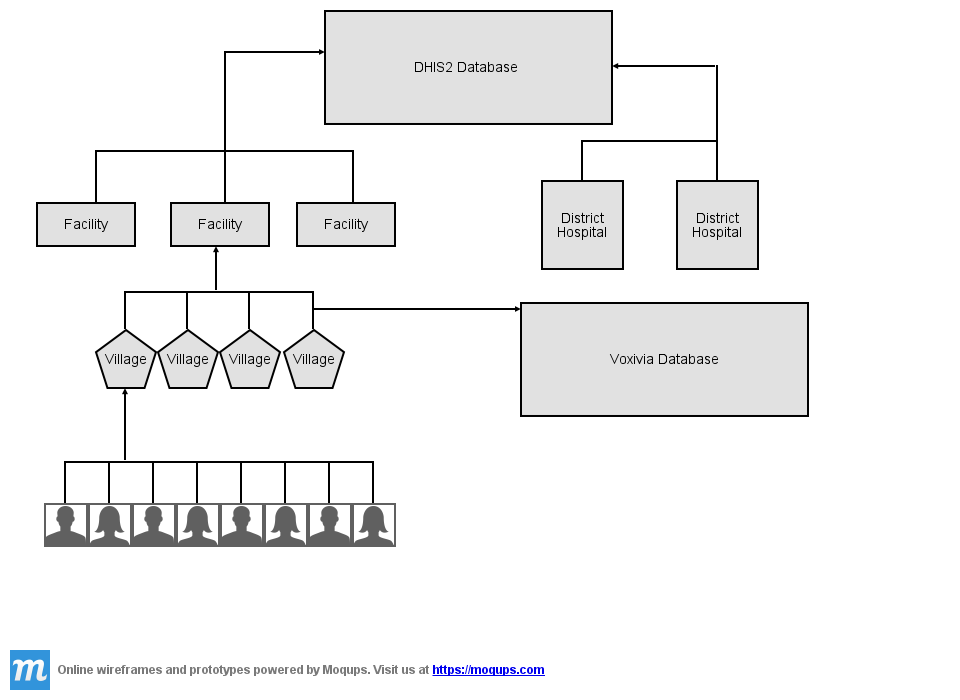
\includegraphics[width=12cm]{empirical/images/dataflow}
\label{dataflow}
\caption{Dataflow}
\end{figure}
In figure \ref{dataflow} you can see how the data flows from users all the way to the DHIS2 database. Actually the data from user all the way up to the health facilities is paper based.
These data flows would greatly benefit from transitioning to an electronic based system. The same is true for the district hospitals. Users usally collects data in a paper based version, but this is currently for conveniance. In the villages there simply isnt an alternative and data from villages is collected and aggregated at the health facilities. This causes a problem. Because all data is aggregated one cannot tell the differance between villages. Currently this is supported by the program offered by Voxivia. For an example, if a village would run out of some drug and another village in the same catchment area would have to much, the will report that the stock of drugs is good. The Voxivia on the other hand would report each village separately and therefore is still in use.
\subsection{Malaria Surveliance}
The malaria surveliance project consists of two main branches. 
\subsubsection{Sentinel Surveliance}
The malaria sentinel project is implemented and is currently reporting weather data and malaria cases, with some extra information.
The purpose of this instance is to map all malaria cases based on their geographical location and see if there is a connection with malaria data and weather data. 
It certainly is. 
\begin{figure}
\centering
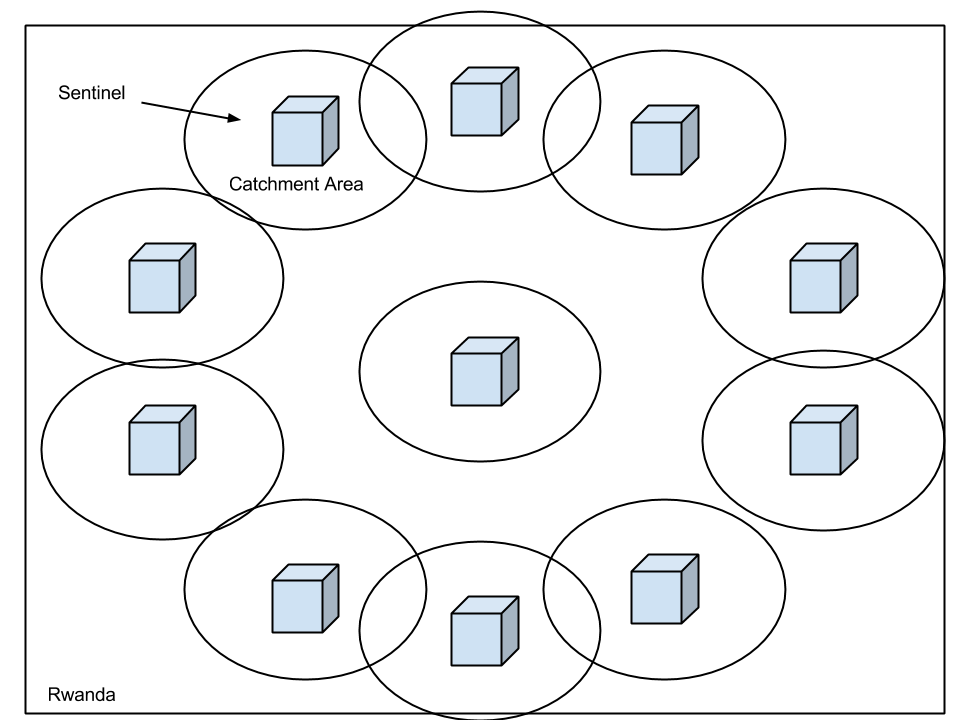
\includegraphics[width=12cm]{empirical/images/sentinel_surveliance}
\label{sentinel_surveliance}
\caption{Sentinel Surveliance}
\end{figure}
The sentinels are differents stations spread throughout Rwanda. Adding up the sentinels catchment area they should cover all of Rwanda. 
Currently these stations data isnt integrated in DHIS2. This is a very simple task, but it needs to be coordinated by the leaders so that everybody is onboard with the solution.
DHIS2 is currently supporting all the requirements, but in order to make the transistion the personell doing the reporting has to be trained.
\subsubsection{Active Surveliance}
Active Surveliance is another branch of the malaria surveliance. The thing is, one wishes for data from the place were the malaria was first noticed.
This kind of data would include if the infected person has bednets, if others in the same house has malaria and other contextual data in hope of seing a pattern to what is most likely to make a person infected. Currently the health personell is using a paper based reporting form, but would like to transition to an electronic based report.
The technology that the health workers currently are equipped with is usally regular simple phones that could interact with DHIS2 with SMS. DHIS2 is supposed to support this feature, but it is not been properly tested. A requirement is that one would have to set up a SMPP\nomenclature{SMPP}{Simple Message Pear-to-Pear} gateway with a local teleoperator. In this case the most likely would be MTN.
The technical expertise for this kind of functionality isnt the main obstacle. It's the bearucracy. The decicion process is long and it takes a while just to map who to talk to about what before one could even start testing.
\subsection{External Systems and DHIX}
\begin{figure}
\centering
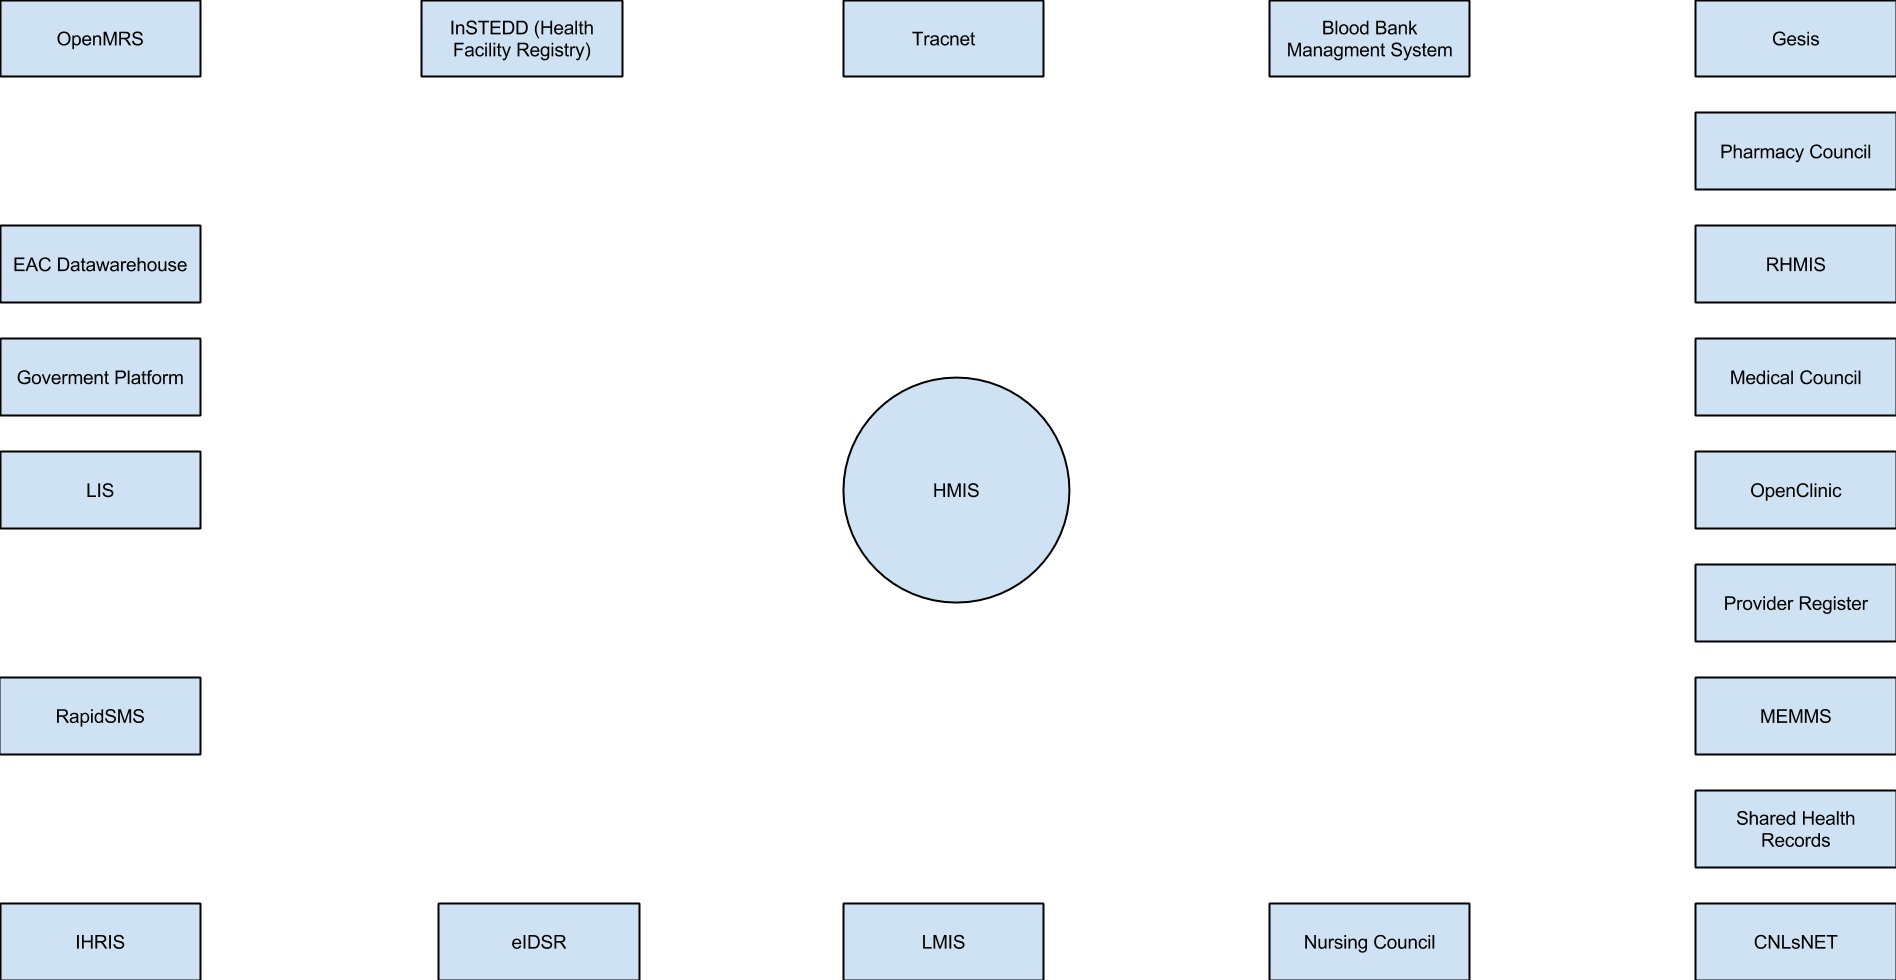
\includegraphics[width=12cm]{empirical/images/context}
\label{external_systems}
\caption{External Systems}
\end{figure}
Figure \ref{external_systems} shows the systems that got mapped during the case study. DHIX represents the HMIS system. The HMIS is currently running four instances of DHIS2 with some scripts for synchronizing data between instances.
\begin{figure}
\centering
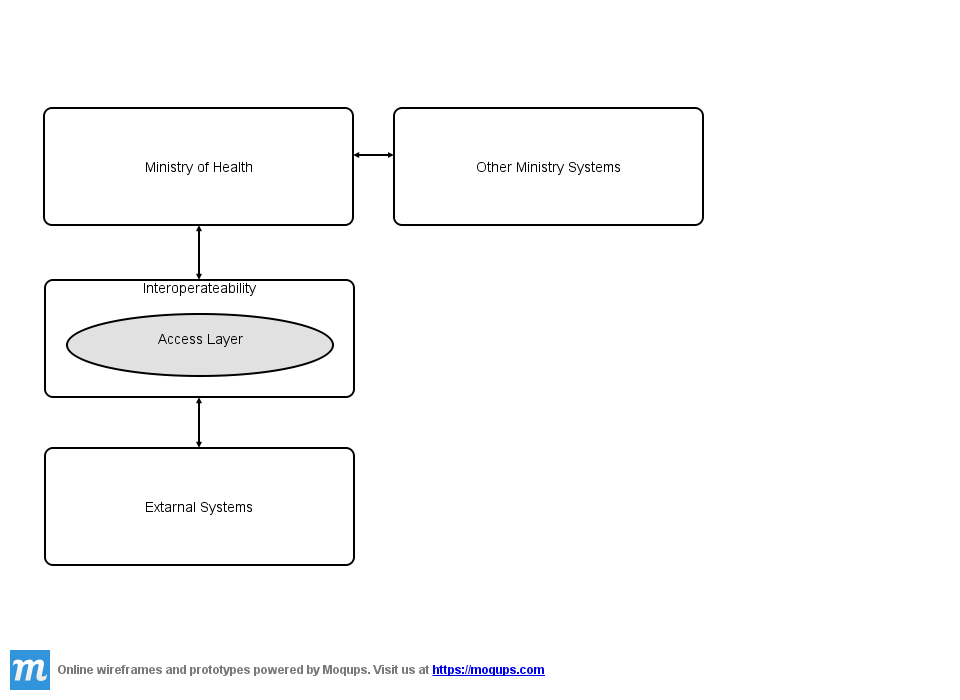
\includegraphics[width=12cm]{empirical/images/future_design_rwanda}
\label{future_design}
\caption{Future Design}
\end{figure}
The HMIS has a vision on how they would like to interact with other systems, see \ref{future_design}. HMIS would like to collect all Ministry of Health systems under one roof. Then they would like to make some kind of interface between health ministry and other ministry systems. The specifics of how this is going to work are not decided yet. The ministry of health would like to be able to exchange data with external systems as well. This is done via an access layer. Between this access layer one would be able to synchronize data with external systems. For instance, there is a system called Voxivia that has data that is more specific than what is currently supported by the DHIS2. These data would be of great benefit to the HMIS. 
\subsubsection{DHIX}
DHIX is the name that we gave the system at the HMIS. As mentioned, this system consists of several subsystems.
\begin{description}
\item[HMIS]General health statistics for Rwanda. 
\item[Health Finance]Contains data for performed health services. Like a treatment program. This data is used for Performance Based Finance, \nomenclature{PBF}{Performance Based Finance}PBF. PBF allocates resources based on how well the facility is performing.
\item[Individual Records]Contains data specific to individuals using the tracker module in DHIS2.
\item[Datawarehouse]This instance has all the important statistics of the other DHIS2 instances.
\end{description}
\begin{figure}
\centering
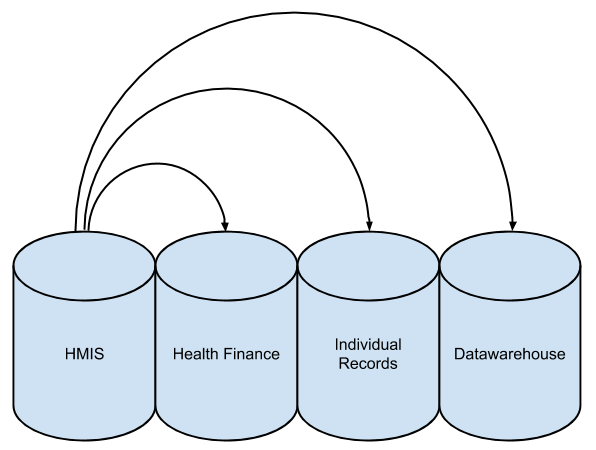
\includegraphics[width=12cm]{empirical/images/hfr_dhix}
\label{hfr_dhix}
\caption{Health Facility Registration in DHIX}
\end{figure}
When it comes to Health Facilities the different systems has to synchronize with eachother. As in figure \ref{hfr_dhix}, the HMIS server should be able to push data to the other instances of DHIS2. In the future, the HMIS would like to make it possible to push data groups into other instances of DHIS2 as well as health facilities.
\subsubsection{Health Facility Registry}
Currently the registration of new health facilities is done on a platform developed by inSTEDD, also known as the HFR\nomenclature{HFR}{Health Facility Registry}. The HMIS is planning to do this registration at the HMIS instance of DHIS2. The inSTEDD platform is used by all external systems that uses the list of Health Facilities, so in order to transition this functionality to DHIS2 all systems that  depends on this service has to be on board. 